\label{ch:related-work}

In this chapter, we present related work and how our approach compares to these. We applied a smooth continuous control reinforcement learning algorithm with amendments for the use in a rotating coordinate space to solve wind turbine load control, hence we evaluate other works solving wind turbine load control with a specific focus on approaches incorporating machine learning. Specifically, works by \citet{coqueletBiomimeticIndividualPitch2020} and \citet{asgharniaLoadMitigationClass2020} fall into this category, and we give a summary of them in Sections \ref{section:related-kotlett} and \ref{section:related-asgharnia}. There is a high number of works solving wind turbine load control without the use of machine learning, we present the work by \citet{jonesOvercomingFundamentalLimitations2018} as a representative in Section \ref{section:related-jones}. Our approach directly builds upon, evaluates against, and competes with the ideas of \citet{bossanyiIndividualBladePitch2003} as presented in Section \ref{section:background-ipc}. Due to the exhausive referencing throughout the rest of the work, we will not reference traditional \ac{IPC} approaches in this chapter. 
% Other works that fall into this category include \todo{spam stuff into this list}:

% \begin{itemize}
%   % \item \citet{bossanyiIndividualBladePitch2003} and \citet{bossanyiFurtherLoadReductions2005} wrote the foundational paper for individual pitch control, discussed in background section \ref{section:background-ipc}
%   \item \citet{larsenActiveLoadReduction2005} propose different input sensors which measure flow as an IPC basis
%   % \item \citet{jonesOvercomingFundamentalLimitations2018} work with local inflow sensors on the blades to improve IPC performance.
% \end{itemize}

% We refrain from summarizing these works, as they are close or comparable to other works presented.

While RL for wind turbine load control has not seen a high amount of published works, other control aims in the field of wind turbines have been researched.
\begin{itemize}
  \item \citet{hosseiniImprovingResponseWind2020} learn PID parameters through \ac{RL} with the aim of output power smoothing
  \item \citet{chenReinforcementbasedRobustVariable2020} stabilize rotor speed through a \ac{RL} collective pitch controller
  \item \citet{zhangReinforcementLearningBasedStructural2020} stabilize floating turbines through \ac{RL}
  \item \citet{saenz-aguirreArtificialNeuralNetwork2019} implement \ac{RL}-based active yaw control
  \item \citet{zhaoCooperativeWindFarm2020} use \ac{RL} for wind farm control
  \item \citet{padullaparthiFALCONFArmLevel2022} use \ac{RL} for wind farm control
\end{itemize}
Each of this works has another optimization goal than our approach, and due to that a different choice of measurements, RL architecture and evaluation metrics. Hence, these works are not in the scope of this chapter.

Lastly, our approach is comparable to any continuous control reinforcement learning applications in a rotating coordinate space, independent of the actual field of application. To us, no such applications in a rotating system are known outside the field of wind turbine control. The more general field of continuous control reinforcement learning applications offers a vast amount of published work, but the intersections with our work are slim and comparability is not given. Hence, this boarder field is out of the scope of this chapter.






% \item \citet{yangIndividualPitchController2016} implement a fuzzy logic based pitch controller
% \item \citet{yilmazPitchAngleControl2009} train a supervised model to match a known pitch signal



% Some examples for further applications of \ac{RL} outside the field of wind turbine control are
% \begin{itemize}
%   \item \citet{leeAlgorithmAutonomousPowerincrease2020} control nuclear power plant startup with \ac{RL} 
%   \item \citet{hwangboControlQuadrotorReinforcement2017} control a quadrocopter through \ac{RL}
%   \item \citet{piLowlevelAutonomousControl2020} control a quadrocopter through \ac{RL}
%   \item \citet{reddyGliderSoaringReinforcement2018} control a glider through \ac{RL}
% \end{itemize}

\section{Biomimetic Individual Pitch Control For Load Alleviation}
\label{section:related-kotlett}

This section evaluates \citet{coqueletBiomimeticIndividualPitch2020}. Their general aim is to reduce wind turbine fatigue loads with an alternative strategy to the common Coleman transformation based IPC. As seen in Figure \ref{fig:coquelet-schema} they utilize a three-level pipeline for their setup. The flow sensing component is a preprocessing component, which evaluates sensory inputs. The central pattern generator transforms the discrete RL signals into continuous individual pitch angles. The \ac{RL} component in the middle outputs amplitude and phase parameters to the oscillators. They utilize the algorithm \ac{SAC} with a discrete action space.

\begin{figure}
  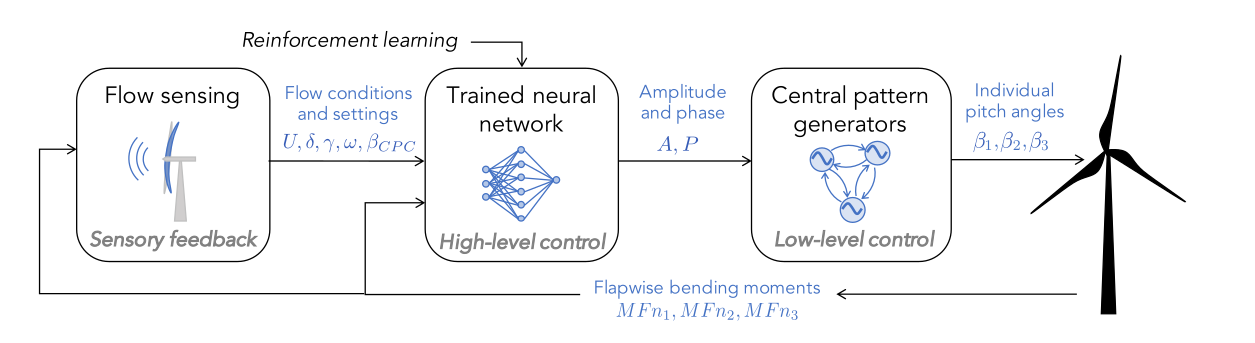
\includegraphics[width=\textwidth]{images/Coquelet-schema.png}
  \caption{The schema of the biometric \ac{IPC} by \citet[Figure 1]{coqueletBiomimeticIndividualPitch2020}}
  \label{fig:coquelet-schema}
\end{figure}

They minimize the distance between the highest and lowest blade bending moment as in equation \ref{eq:coquelet-reward}:
\begin{equation}
  r(s, a) = (\max_i(\soopbend_i) - \min_i(\soopbend_i)^{-2}
  \label{eq:coquelet-reward}
\end{equation}

Their training environment consists of a lower accuracy \ac{BEM} model of the wind turbine, while their evaluation happens in a higher quality \ac{VPM} based simulation. They test on the NREL 5MW reference turbine \cite{jonkmanDefinition5MWReference2009}. Instead of directly outputting pitch angles, the \ac{RL} agent outputs phase and amplitude settings for biometric oscillators which generally follow the form of equation \ref{eq:coquelet-oscillator}:

\begin{equation}
  \ddot{x} = \kappa_x (\frac{\kappa_x}{4}(X - x) - \dot{x})
  \label{eq:coquelet-oscillator}
\end{equation}

where $x$ is the output from the \ac{RL} agent, $\kappa_x$ is a gain constant, $X$ is a target value for $x$ to smoothly converge to and $\dot{x}$ and $\ddot{x}$ being the first and second derivative of the variable. This formula is used to compute offset, amplitude and phase of a oscillation: $\apitch = x_{\text{offset}} + x_{\text{amplitude}} \cos(x_{\text{phase}} + \sazi)$. While amplitude and phase are output from the \ac{RL} agent, the offset is taken as the pitch output from a traditional collective pitch controller.

\begin{figure}
  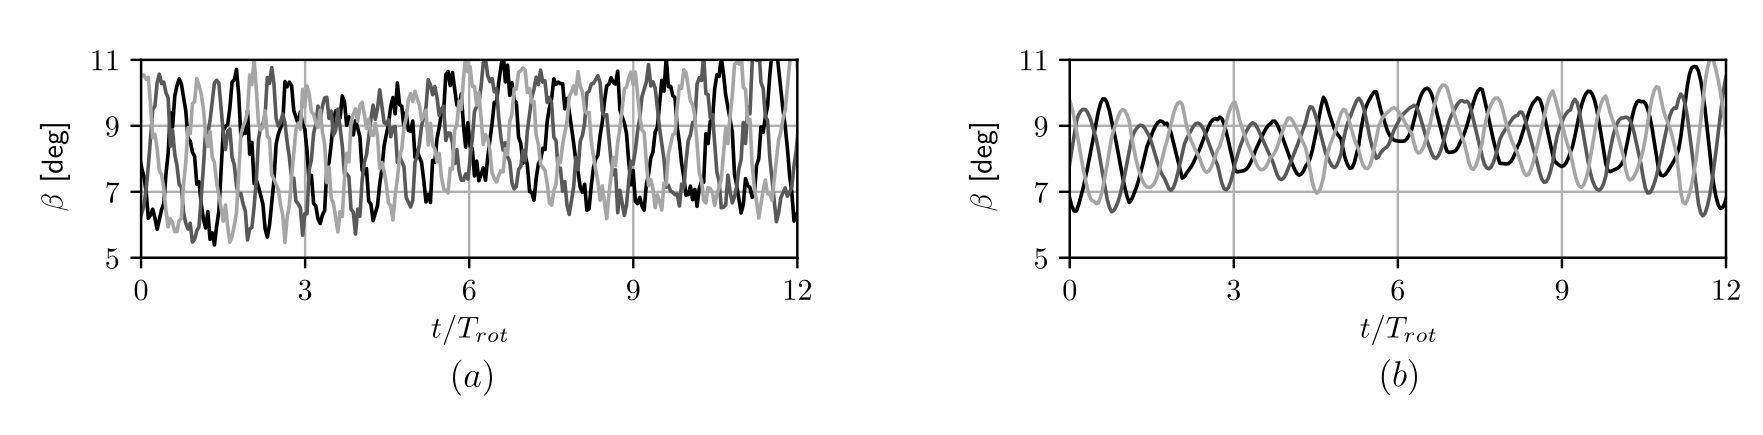
\includegraphics[width=\textwidth]{images/Coquelet-results.png}
  \caption{A rollout of a traditional Coleman-Transform based IPC (a) versus their biometric \ac{IPC} (b) by \citet[Figure 5]{coqueletBiomimeticIndividualPitch2020}}
  \label{fig:coquelet-results}
\end{figure}

\begin{table}
  \centering
\begin{tabular}{c c}
\hline
Method & Equivalent bending moments [MNm] \\
\hline
CPC & 2.54 \\
CT-IPC & 0.99 \\
BI-IPC & 1.40 \\
\hline
\end{tabular}
\caption{Equivalent bending moments from a collective pitch controller (CPC), a Coleman-Transformation based IPC (CT-IPC) and their biometric IPC (BI-IPC), by \citet[Table 1]{coqueletBiomimeticIndividualPitch2020}}
\label{table:coquelet-results}
\end{table}

To evaluate their results, they calculated equivalent bending moments, a measure which calculates a material-specific fatigue load equivalent to a seen trajectory \cite{blasquesMeanLoadEffects2013}. In Table \ref{table:coquelet-results}, their results show that their biometric IPC reaches less fatigue load reduction than a Coleman-Transformation based IPC but more than a collective pitch controller. They argue however, that their rollouts are smoother than the IPC as seen in Figure \ref{fig:coquelet-results}, thus forming a compromise between the CT-IPC and CPC. Furthermore, they claim more input information such as local blade flow velocities to allow for further blade load reduction, but do not show experiments to prove this.

\subsubsection{Direct Comparison}

This work is similar to our work in many terms. It uses similar methodology and similar inputs to solve the same problem. However, they optimize a different turbine model and different wind inflow conditions, hence direct comparability is not necessarily given.  As in our work, they use the reinforcement learning algorithm \ac{SAC} and utilize common wind turbine sensors as neural inputs. In contrast to our approach, they incorporate wind flow information. Compared to our results, they achieve less strong blade load reductions but also less strong pitch load increases, hence they trade pitch and blade loads differently. This is due to several factors.

Firstly, they operate in a discrete action space. While policies in a discrete action space tend to easier to train, they lack expressivity. It requires significant post-processing efforts to translate discrete actions to continuous smooth pitch angles. They utilize biometric oscillators to perform this translation. These oscillators produce gentle and smooth outputs even with a discrete input, but the possibilities of the reinforcement learning agent are limited strongly. Developing a pitching strategy with rich spectral contents on high frequencies, as observed in our work, is inhibited by the smoothing of the biometric oscillators. Operating directly in the continuous space like in our work offers more flexibility regarding the learnt policy. 

Secondly, they utilize a linearized model of the wind turbine to train their policy and a simulated environment to evaluate. By using the linearized model for training, they trade lower training complexity for lower learning potential. The partially non-linear aspects of the wind-turbine model are masked away, and some optimization potential is lost.

Third, they utilize a reward function which we briefly revisited during our experimentation. They penalize the squared difference between the highest and smallest bending moment, effectively incentivizing the bending moments to stay close to each other in each time frame. This does not penalize poor mean bending moments. For example low frequency oscillations, where all bending moments oscillate together on the tower eigenfrequency, are undetected by this reward. Also, extreme loads are undetected. However, due to the few terms, their reward function is compact and likely easier to learn than ours.

Congruent to our findings they conclude that RL is in principle able to optimize the wind turbine environment. Through the heavy filtered biometric oscillators, their policy is constrained to smooth actions and has less potential of damaging but also less potential of optimizing the turbine than in our work. In contrast to us, they do not outperform their IPC baseline with respect to the primary optimization metric blade loads.

\section{Load Mitigation Of A Class Of 5-MW Wind Turbine With RBF Neural Network
Based Fractional-order PID Controller}
\label{section:related-asgharnia}

This section evaluates \citet{asgharniaLoadMitigationClass2020}. They build a set of different PID-based collective pitch controllers for the NREL 5MW reference turbine \cite{jonkmanDefinition5MWReference2009} and evaluate them with respect to different metrics. In traditional controller design, a linearized model of the wind turbine is assumed and used as a tuning reference for PID parameters. Due to the linearity of the model, a closed form solution to the PID parameters can be found \cite[Eq 12 - 22]{asgharniaLoadMitigationClass2020}. This closed form solution yields different results for different operating wind speed, i.e. the optimal set of parameters to a PID controller depends on the speed of the incoming wind.

They build upon a common technique in wind turbine control design called gain scheduling. For this, a different set of parameters $(K_p, K_i, K_d)$ is used for different wind speeds. Obtaining robust wind speed measurements is nontrivial, as direct wind speed measurements by an anemometer are noisy. Anemometers are usually placed downstream of the rotor and thus experience wake effects from the passing blades. Furthermore, they only offer a point estimate of the wind speed at the nacelle, while the speed at the blade tips can be very different. Thus, they train a Radial-Basis-Function Neural Network to output the correct set of PID parameters based on wind turbine state. Concretely, they use rotational speed, output power and pitch angle. This training happens in a supervised fashion, as the wind turbine state for a given wind speed is known and the wanted PID parameters for a set of wind speeds were computed beforehand. Additionally, they utilize fractional order PIDs, which are similar to traditional PID controllers but with an additional parameter to the integration and derivation constant \cite[equation 24]{asgharniaLoadMitigationClass2020}.

They evaluate with respect to generator error (how far the generator output deviates from a wanted setting), pitch actuation, tower fore-aft torque and out-of-plane blade bending moments. For each scenario, they calculate \ac{RMS} values for their metrics in five different wind speeds with different wind noise levels. Their top performing variant, the FOPID showed 19.3\% less generator error than a baseline PID without a neural network, 22.4\% less pitch actuation rate, 13.3\% lower tower fore-aft acceleration and 19.7\% less out-of-plane bending moment. With this, they significantly outperform the baseline collective pitch controller, showing that a more intelligent actuation strategy has the potential of reducing blade, tower and pitch actuator loads at the same time. The \ac{RMS} metric is not directly comparable with other works like \citet{coqueletBiomimeticIndividualPitch2020} or \citet{bossanyiFurtherLoadReductions2005}, which calculate \acp{DEL}. However, it can be assumed that this collective strategy is an improvement over previous collective strategies. A collective pitch strategy has the advantage of being applicable to turbines which can not actuate their blades individually. Furthermore, it is imaginable to combine the FOPID with a load minimizing IPC, further reducing blade loads at the expense of extra pitch travel. 

\subsubsection{Direct Comparison}

In contrast to this work, this work does not utilize reinforcement learning, but a supervised framework to train a neural network to set PID parameters. Supervised learning is less complex, as it does not have to perform value approximation to then derive a policy from it, but directly uses human knowledge about optimal outputs based on wind turbine operating state inputs. This allows easier analysis of the approach and more security for real world applications. However, security guarantees are lower than those of traditional PID based works which can calculate a safety margin in closed form, as the neural network is still essentially a black box. The results are not directly comparable to our work due to two factors, first the use of a different evaluation metric, but more importantly, the fact that their work tackles collective pitch control instead of individual pitch control. Expected load reductions of collective pitch are significantly lower than those of individual pitch control at the benefit of reduced actuation complexity. Furthermore, a CPC policy can not reduce asymmetric rotor loads, while an IPC policy can. This difference makes a direct comparison of loads unsuitable. More generally, it can be stated that the use of machine learning techniques has leveraged higher optimization yields in this case, similar to our results.


\section{Overcoming Fundamental Limitations Of Wind Turbine Individual Blade Pitch Control With Inflow Sensors}
\label{section:related-jones}

This section evaluates the work of \citet{jonesOvercomingFundamentalLimitations2018}. Though this is not based on machine learning, it is a very promising method for load reduction.

Their key selling point is an \ac{IPC} design based on additional blade-local lift estimations. These lift forces can be inferred from pressure measurements using pitot tubes in the blades, effectively measuring local angle of attack and incoming air speed. When a gust hits the blade, these sensors immediately detect the higher load and can initiate a pitch reaction earlier than possible for a normal IPC. A normal IPC has to wait until the bending moments are at a high enough level to trigger a PID response, which is a long time on a modern wind turbine. Through a cascaded IPC design, which adds extra pitch actions inferred from inflow sensors to the IPC actions, they reach faster reaction times and stronger reactions.

The cascaded IPC exhibits better blade wear than the state-of-the-art, reducing blade DELs by ca 10\% in turbulent wind compared to their IPC baseline, but at the expense of higher pitch travel. The impact on extreme loads is relatively large, reducing maximum loads during an example wind shear by a factor of 2.5 with increased pitch travel by a factor of 2. 

\subsubsection{Direct Comparison}

A direct comparison is difficult, as they evaluate a single design load case with a wind shear and we evaluate in turbulent and steady wind. Through the single load case, load reductions are difficult to assess, as the load case could be not representative of a turbine life. However, their cascaded IPC exhibits lower blade loads at the cost of higher pitch travel, which is similar to our result. In the design load case shown, they reach a significant extreme load reduction an order of magnitude above the reduction provided by WINDL on average.

The authors argue that \ac{BRBM} sensors do not exhibit enough bandwidth to reach higher blade load reductions through the \ac{IPC} strategy, and other sensors like inflow sensors are needed instead. We show in our work that a non-linear neural policy is able to achieve further blade load reductions without using inflow sensors sensors but only using traditionally installed sensor inputs. In our case, these advancements have to do with the way the information is processed in the controller, hence we are able to overcome the fundamental bandwidth limitation partially. We assume that through the integration of advanced sensors like inflow sensors, also the WINDL policy could be improved as it receives more information about the surrounding flow.

Through the PID based IPC design, they can calculate a mathematical safety margin, whereas the WINDL policy can only be evaluated empirically to be safe. Such a safety margin is an important guarantee and likely a critical factor towards real world adoption.